\section{Results}

The highest ranking features for differentiating Gleason scores are summarized
by texture extraction method in Table~\ref{tab:texture_best1p}. Features based
on Gabor filters were included in all image types. GLCM features were selected
for T₂w and T₂, and Zernike moments for K and T₂. Features from the Hu
moments and LBP were also selected for T₂, in which the top 1\% had more
variability than other image types, regarding both the texture extraction method
and window size.


\subsection{Univariate Analysis}

ROC analysis was performed for each texture feature. The resulting best features
are shown in Table~\ref{tab:texture_imagetype}. The best one was MBB-GLCM
homogeneity in T₂w with AUC=0.84.

A similar analysis was performed for the first-order statistical features;
results are shown in Table~\ref{tab:stats_imagetype}. Although the best
statistical features had good performance for most of the modalities, they did
not out-perform the best texture features.

Some of the high-ranking features are visualized in Fig~\ref{fig:tmap}. In
addition, ROC curves for best statistical and texture features are presented in
Fig~\ref{fig:roc}.

\begin{figure}[htb]
\centering 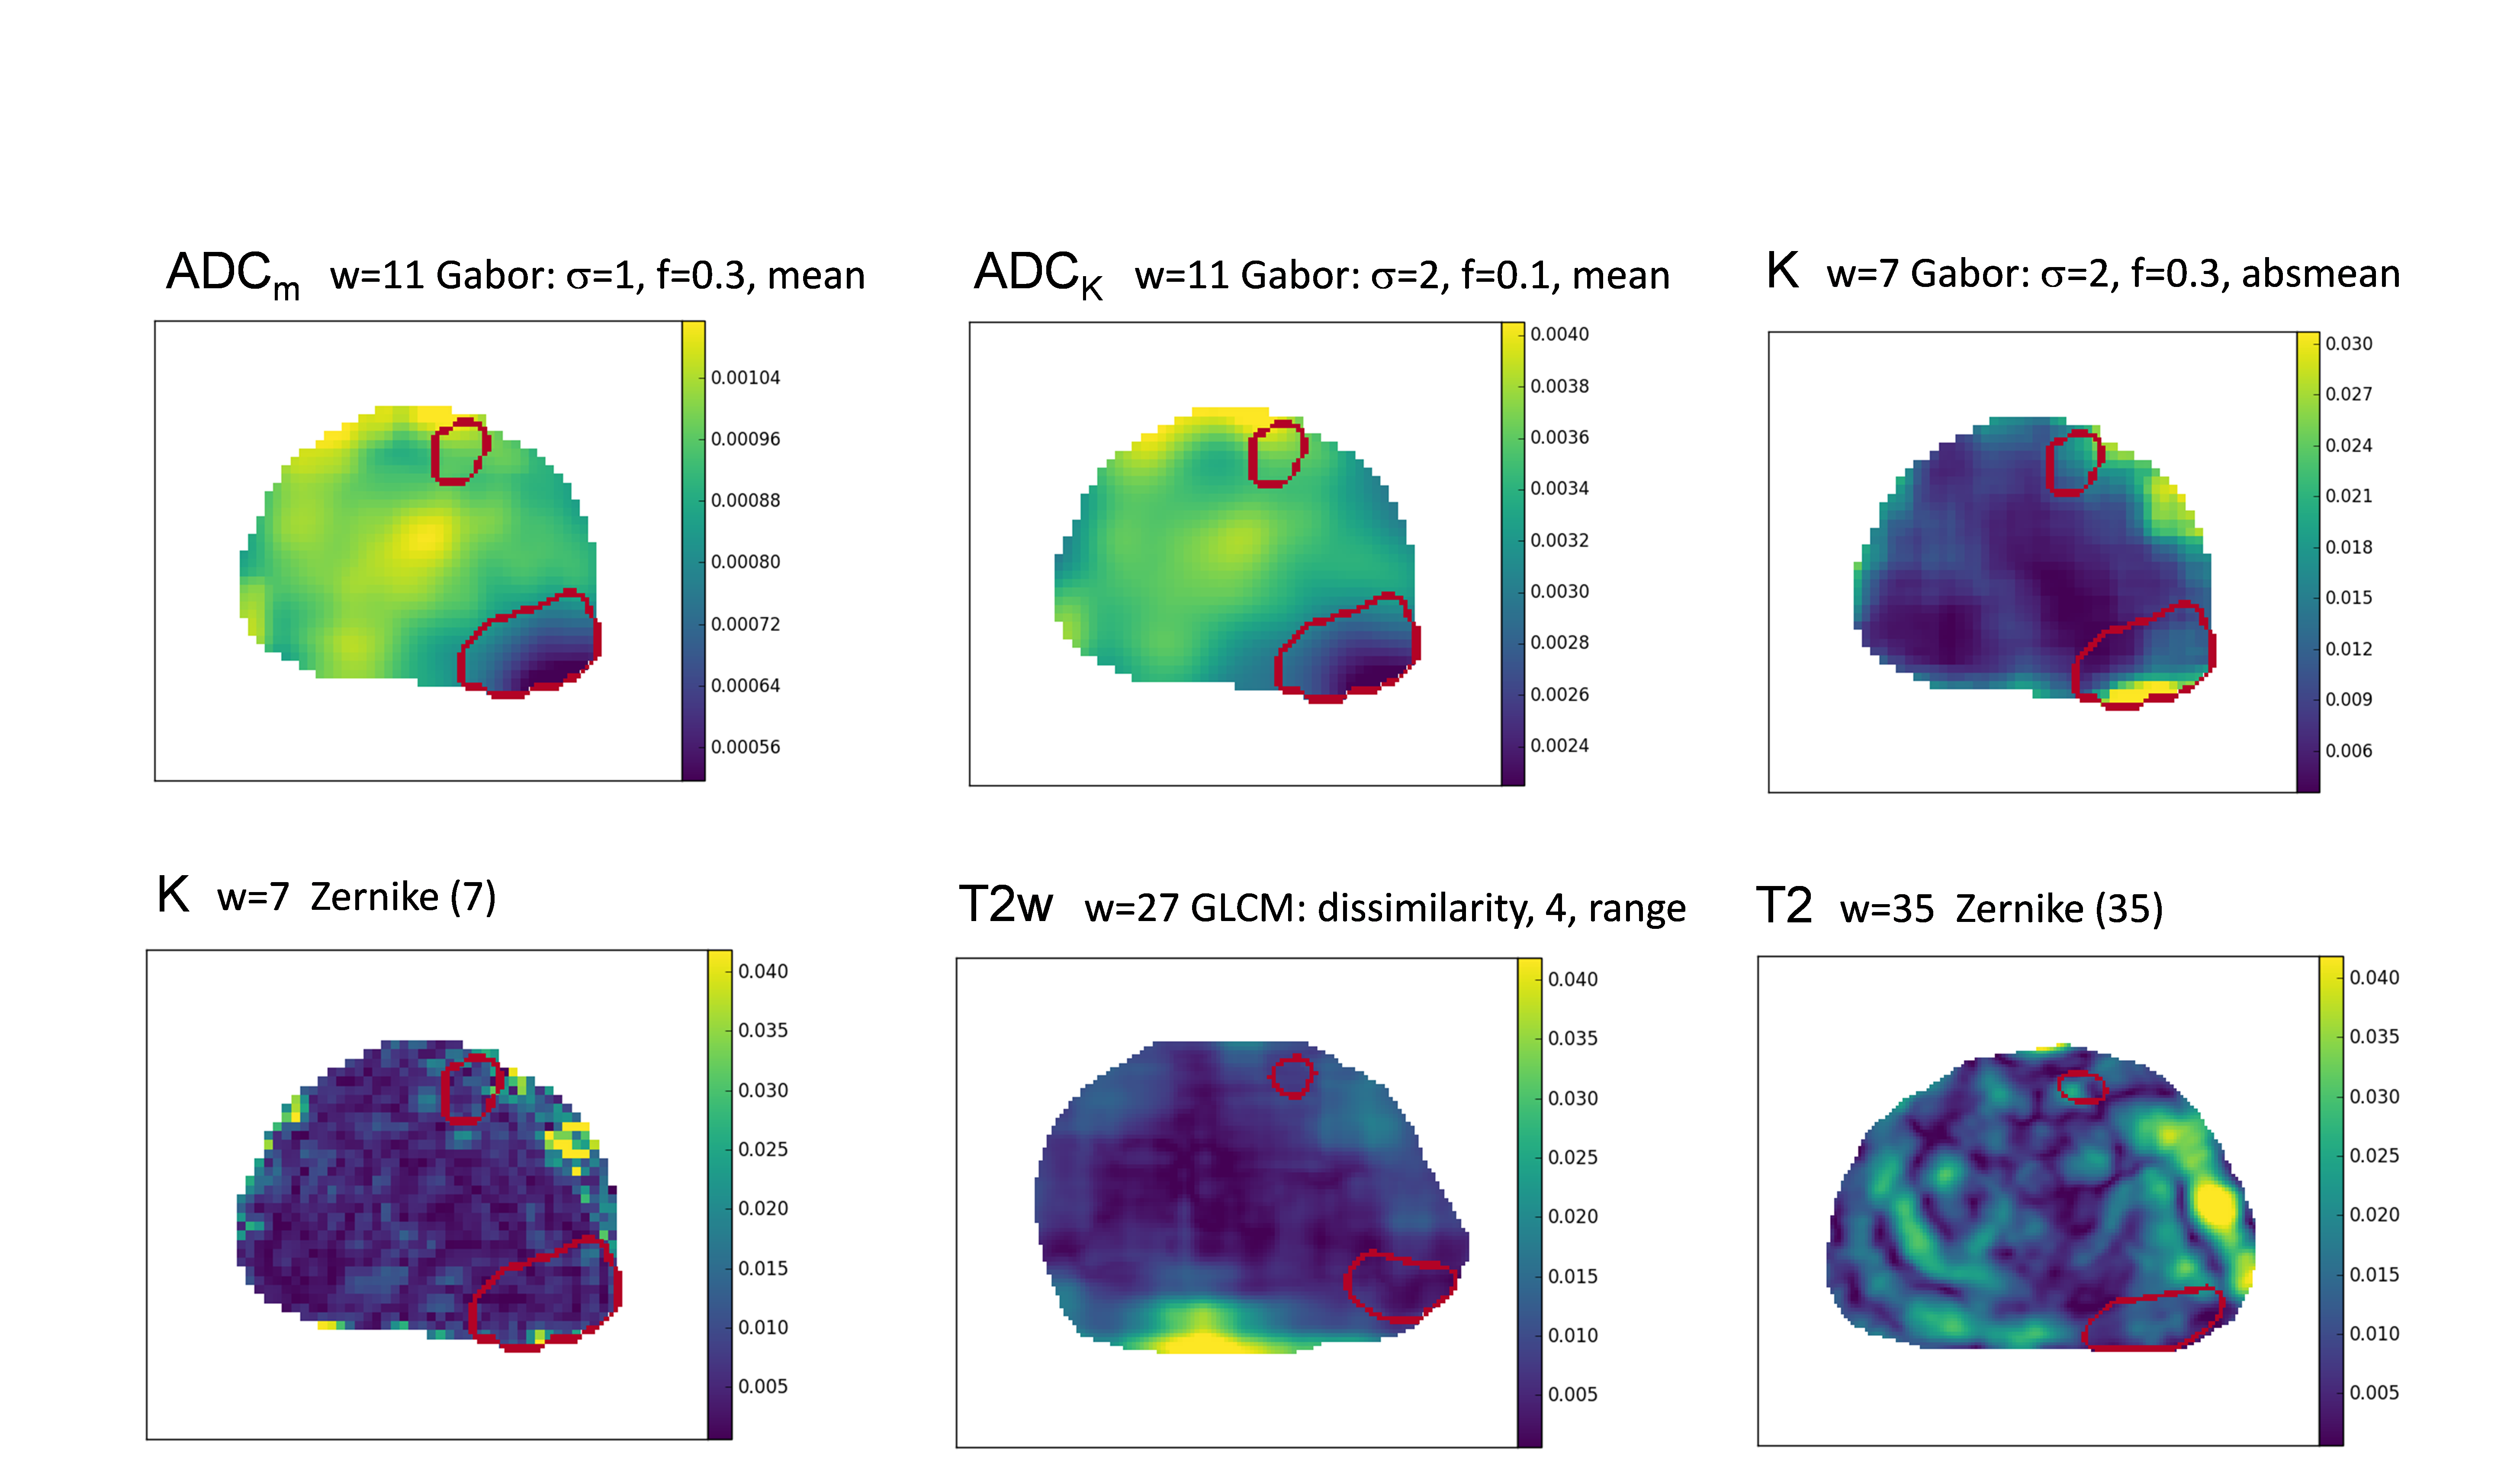
\includegraphics[width=1.0\textwidth]{figures/fig3}
\caption{An example of prostate texture feature maps extracted from DWI
parametric maps (ADCₘ, ADCₖ, K), T₂-weighted imaging (T₂w), and parametric map
of T₂ relaxation values (T₂). Source image type, window size, and texture
descriptor parameters are shown above the images. The two lesions are outlined;
their Gleason scores are 4+3 (lower) and 3+4 (upper).}\label{fig:tmap}
\end{figure}

\begin{figure}[htb]
\centering 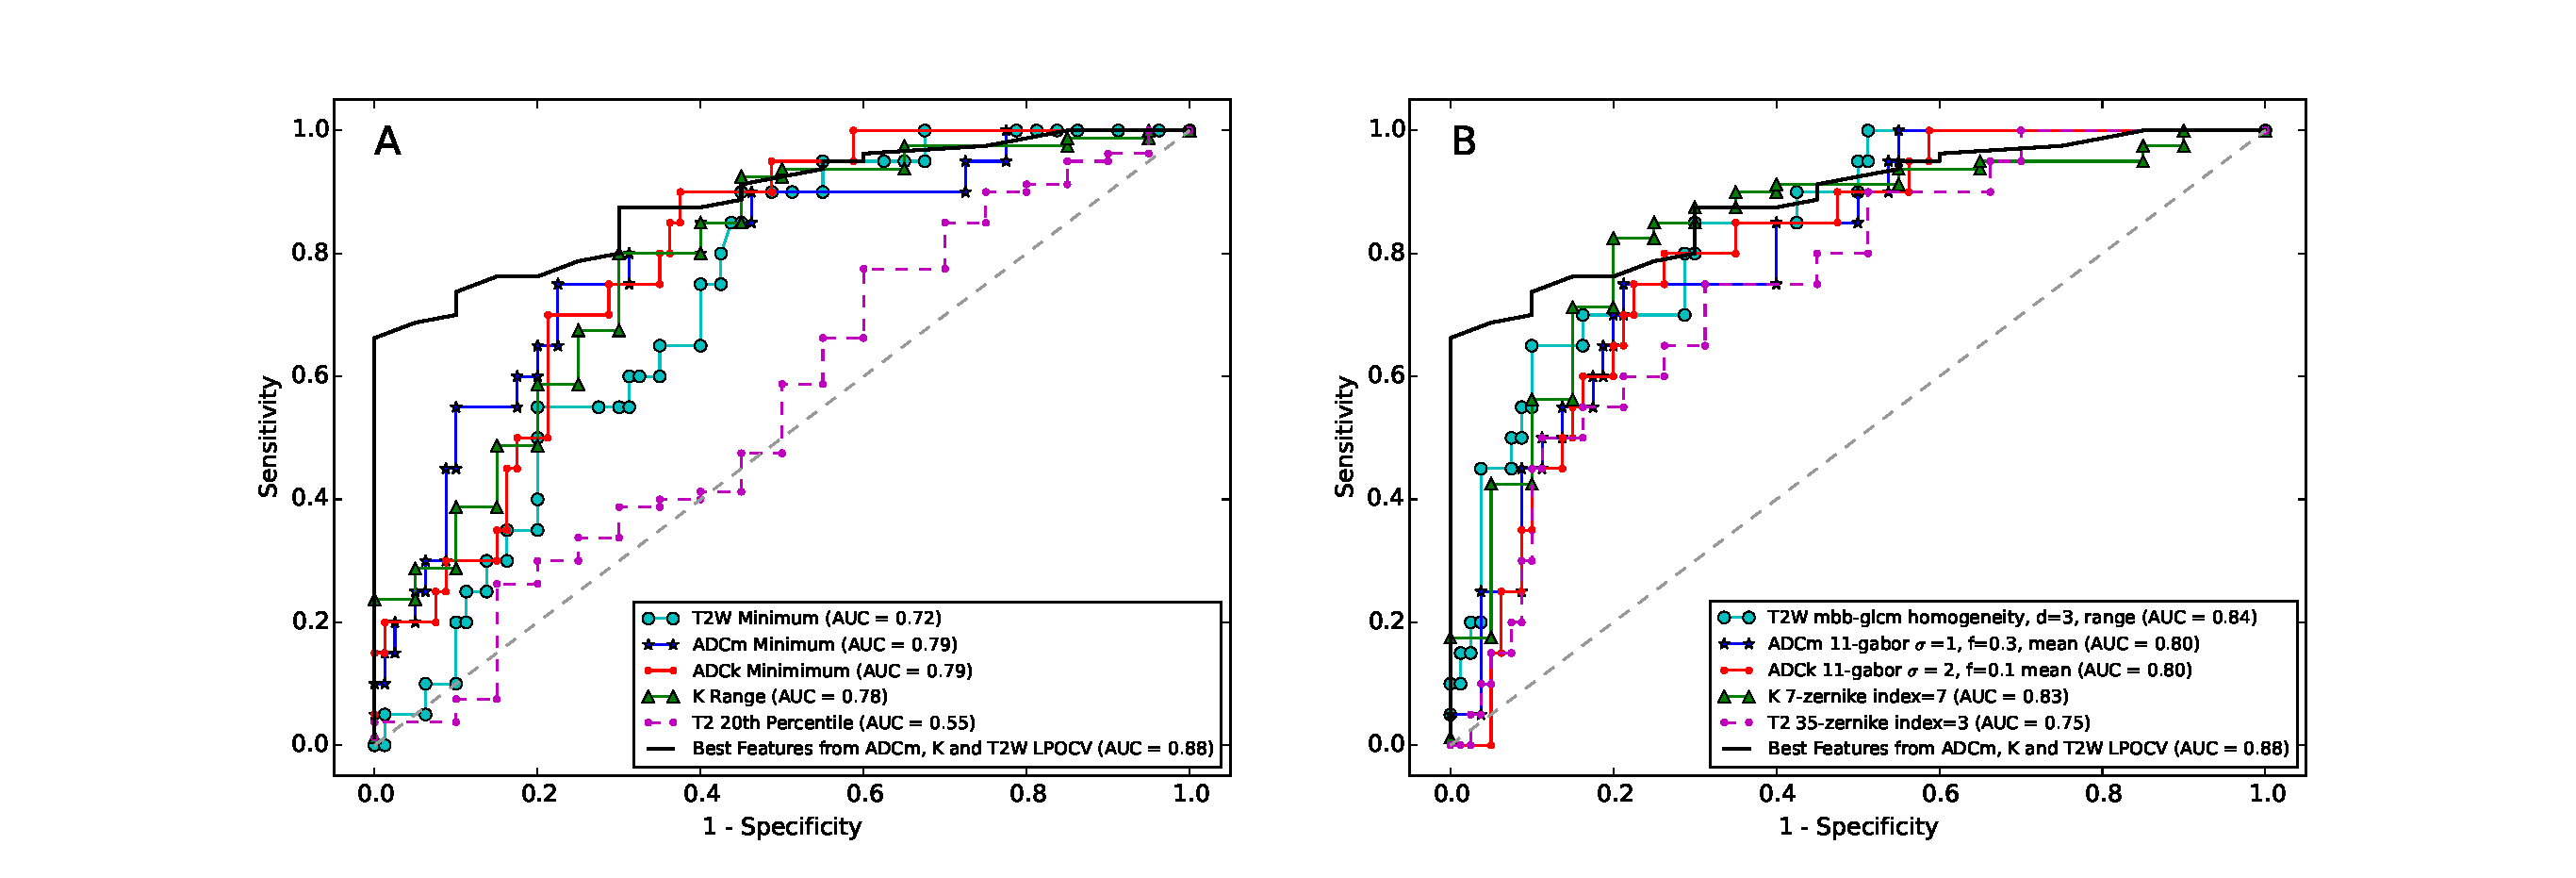
\includegraphics[width=1.0\textwidth]{figures/fig4}
\caption{The ROC curves for the best statistical feature (A) and the best
texture feature (B) within each image type (T₂w, ADCₘ, ADCₖ, K, T₂). The final
model of the best selected features from ADCₘ, K, and T₂w obtained using L1
regularized logistic regression and validated with leave-pair-out
cross-validation (LPOCV) is also included in both A and~B.}\label{fig:roc}
\end{figure}


\subsection{Multivariate Analysis}

The prediction performance of the models trained using regularized logistic
regression was estimated by LPOCV\@. Both L1 and L2 regularization methods were
utilized separately. Table~\ref{tab:auc_imagetype} contains the results for
models within each image type using all of the features and top 1\% of them. The
results are presented as ROC AUC values along with 95\% confidence intervals.

Similar performance estimates of the models combining features from different
image types are presented in Table~\ref{tab:auc_combinations}.


\subsubsection{All features within individual image types}

When using all features and L1 regularization (Table~\ref{tab:auc_imagetype}),
T₂w had AUC=0.82, DWI derived parametric maps (ADCₘ, ADCₖ, K) had AUC range
0.64--0.71, and T₂ derived features had AUC=0.58.

In contrast to L1, L2 regularization yielded better performance for all image
types except T₂w where AUC dropped to 0.68. DWI-derived parametric maps (ADCₘ,
ADCₖ, K) had AUC range 0.69--0.73, and T₂ derived features had AUC=0.70.

These results indicate that, when it comes to logistic regression models, all
features weighted by L2 regularization may perform better than fewer features
selected by L1, with the exception of T₂w images. With T₂w, L1 regularization
performed better than L2, suggesting that a subset of features would perform
better than all of them.


\subsubsection{Selected features within individual image types}

The feature selection was based on filtering features by AUC\@. Only the best
1\% of features (12 or 16 features, depending on image modality) with highest
ranking AUC were selected in each image type. When using L1 regularization, the
best T₂w features showed better performance (AUC=0.80) than the features of
DWI-derived parametric maps (ADCₘ, ADCₖ, K), which had AUC range 0.71--0.78. The
best T₂ features had AUC=0.51 which is the lowest performance among the
modalities.

The estimated AUC values using L2 regularization and the best 1\% features,
compared with L1 regularization, were lower for T₂w and K.

The texture features did not substantially out-perform the 18 statistical
features the corresponding image type (Table~\ref{tab:auc_imagetype}), except in
T₂w where the texture feature model obtained with L1 regularization had the best
performance among all other models. The highest AUC value based on statistical
features was 0.79, achieved using L1 regularization and ADCₘ. The corresponding
value for the best 1\% texture features was 0.71.

The AUC values for the top-1\% texture features based on T₂w, ADCₘ, ADCₖ, K,
and T₂ are shown in supporting material Tables S2, S4, S6, S8, and S10,
respectively. Similarly, AUCs for the statistical features for each image
type are shown in supporting material Tables S3, S5, S7, S9, and S11.


\subsubsection{All features of combined image types}

No substantial improvements of AUC values were present when combining all
features of all image types (Table~\ref{tab:auc_combinations}). The AUCs were
within range 0.53--0.82 with L1 regularization and within 0.69--0.80 with L2.


\subsubsection{Selected features of combined image types}

In contrast to the use all features, a better model performance was present when
combining the best 1\% features of all image types (T₂w, ADCₘ, ADCₖ, K,
T₂). The best performing model with AUC=0.88 was obtained when selecting the
best 1\% features based on ADCₘ, K and T₂w. The combinations of features
extracted from DWI parametric maps (ADCₘ, ADCₖ, K) and those extracted from T₂w
and T₂ together with the feature selection method lead to improved prediction
performance regardless of the regularization method (L1, L2).

The final model proposed to differentiate low from high Gleason score PCa
includes the features from ADCₘ, K, and T₂w listed in Table~S12. The expected
performance ROC is presented in Fig~\ref{fig:roc}.
